% Create a beamer file with cool style.

\documentclass[tikz]{beamer}
\usetheme{Madrid}
\usecolortheme{seahorse}
\usefonttheme{serif}
\useinnertheme{rectangles}
\useoutertheme{infolines}

% We present in english
%\usepackage[swedish]{babel}
\usepackage[utf8]{inputenc}
\usepackage{
	listings,
    graphicx,
    hyperref,
    pgfgantt,
    xspace,
    xstring,
}
\usetikzlibrary{chains,shadows.blur}

\newcommand{\stoe}{S$^2$E\xspace}

\begin{document}
\year=2023
\month=5
\day=26

\title{AMBA}
\subtitle{Interaktiv visualisering av symbolisk fuzzing}
\author{
	\mbox{Loke Gustafsson} \and
	\mbox{Samuel Kyletoft} \and
	\mbox{Enayatullah Norozi} \and
	\mbox{Albin Otterhäll} \and
	\mbox{Clara Salberg} \and
	\mbox{Linus Wallman}
}
\date{\today}

\frame{\titlepage}


\begin{frame}
	\frametitle{hello world}

	hello world
\end{frame}



\begin{frame}
	% Some examples of binary analysis methods are: 
	% binary debugging, which might be a little too manual in many cases;

	% Studying disassembly or decompiling using heuristics and meta data to
	% generate a higher level pseudocode;

	% fuzzing, generating different inputs and studying the outcome of the
	% program, like a crash;

	% Symbolic fuzzing, which we will get to.

	% All methods have their pros and cons and are applicable in different situations.
	% Binary debugging and studying disassembly or decompilation could be very
	% manual and burdenful for the analyst, but it could also give a very good
	% abstract understanding of the program.

	% Fuzzing is an automatic method and requires no interaction, but it doesn't
	% give any abstract understanding of the program. Only determining some
	% inputs satisfying user defined objectives. Like determining crashes,
	% detecting memory leaks and so on.

	% Another problem with fuzzing is the testcase generation. It is not trivial
	% how to generate test cases which effectively covers a large set of
	% execution paths so that no same paths are unneccessarily tested multiple
	% times, or reachable paths that were not explored.

	% The specific problem of test case generation is solved by symbolic fuzzing
	% which relies on symbolic execution.

	\begin{columns}[t]
		\begin{column}{0.5\textwidth}
			\begin{itemize}
				\item Binary debugging
				\item Disassembly
				\item Decompilation
				\item Fuzzing
				\item Symbolic fuzzing
			\end{itemize}
		\end{column}
		\begin{column}{0.5\textwidth}
			
\includegraphics[width=0.3\textwidth]{assets/GDB_Archer_Fish_by_Andreas_Arnez.svg.png}
			\footnote{\tiny by Andreas Arnez, \href{https://creativecommons.org/licenses/by-sa/3.0/us/deed.en}{CC BY-SA 3.0 us}}

			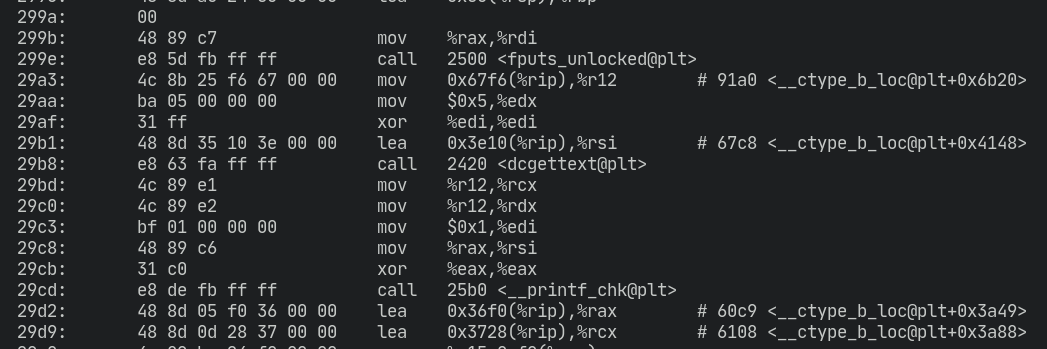
\includegraphics[width=\textwidth]{assets/disassembly.png}

			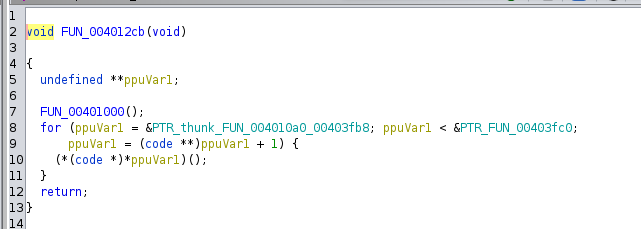
\includegraphics[width=\textwidth]{assets/decompil.png}

			\tiny{
				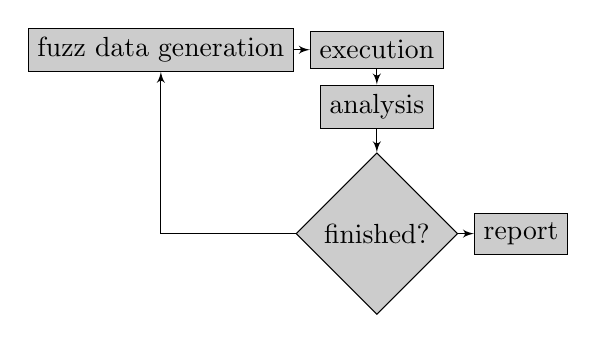
\begin{tikzpicture}

					\node [draw, fill=lightgray!80, minimum height=0.3cm]
					(first) {fuzz data generation};

					\node [draw, fill=lightgray!80, minimum height=0.3cm, right=0.2cm of first]
					(second) {execution};

					\node [draw, fill=lightgray!80, minimum height=0.3cm, below=0.2cm of second]
					(third) {analysis};

					\node [diamond, draw, fill=lightgray!80, minimum height=0.1cm, below=0.3cm of third]
					(fourth) {finished?};

					\node [draw, fill=lightgray!80, minimum height=0.3cm, right=0.2cm of fourth]
					(fifth) {report};

					\path [draw, -latex'] (first) to (second);
					\path [draw, -latex'] (second) to (third);
					\path [draw, -latex'] (third) to (fourth);
					\path [draw, -latex'] (fourth) to (fifth);
					\path [draw, -latex'] (fourth) -| (first);

				\end{tikzpicture}
			}
		\end{column}
	\end{columns}
\end{frame}


\begin{frame}
			\textbf{Symbolic Fuzzing}
	        \vspace{1.8mm}
			\small
			\begin{itemize}
				\item Explore execution paths
				\item Symbolic representation
				\item Tracking conditions into symbolic expressions
				\item Reduces the number of testcases needed
			\end{itemize}
\end{frame}

\begin{frame}
    \vspace{3.0mm}
    \textbf{State explosion}
    \begin{center}
        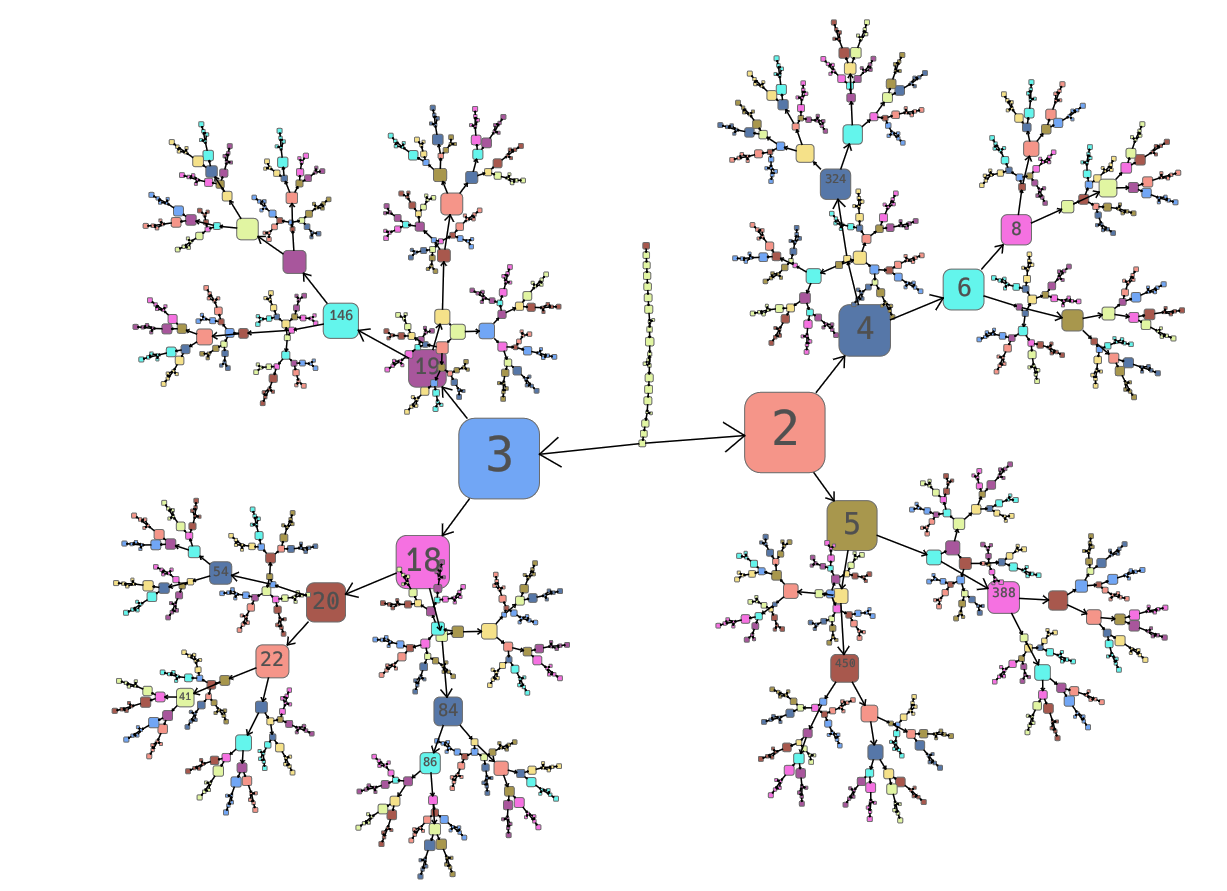
\includegraphics[width=0.95\textwidth]{assets/state-splitter-alpha.png}
    \end{center}
\end{frame}


\section{AMBA}


\begin{frame}
	\centering
	\huge
	DEMO
\end{frame}


\begin{frame}

	\centering
    AMBA is cool, but not useful for real programs

\end{frame}

\begin{frame}

	\centering
    AMBA is cool, but not (yet) useful for real programs

\end{frame}

\begin{frame}

    \textbf{Why is it cool?}
    \vspace{1.8mm}

    In general:

    \begin{itemize}

        \item \underline{Visualized} symbolic fuzzing $\rightarrow$ Human domain

        \item Visualized \underline{symbolic fuzzing} $\rightarrow$ Computer's
            domain

        \item Human $+$ Computer $\rightarrow$ More powerful analysis possible

    \end{itemize}

\end{frame}
\begin{frame}


    \textbf{Why is it cool?}
    \vspace{1.8mm}

    AMBA vs other tools:

    \begin{itemize}

        \item Very few other tools exist. We know of one targeting machine code
            (SymNav). None based on \stoe{}

        \item System virtualization within QEMU through \stoe{}
            \begin{itemize}

                \item Realistic execution environment

                \item Easily extended to multi-process analysis

                \item Maybe kernel, device drivers?

            \end{itemize}

        \item Higher performance ceiling

        \item Real time architecture. No batching

    \end{itemize}

    \pause
    BUT!

    \pause
    AMBA needs
    \begin{itemize}
        \item polish, quality-of-life features

        \item real-world testing \& feedback incorporated

    \end{itemize}

\end{frame}


\begin{frame}[fragile]

	\begin{columns}[t]
		\begin{column}{0.4\textwidth}
			\textbf{Possible improvements}
			\small
			\begin{enumerate}

				\item Implementing state merging

				\item Implementing syscall tracing

				\item Testing on real-world programs

				\item Dynamic symbolic input creation (time, \texttt{stdin}
				      length, etc)

			\end{enumerate}
		\end{column}
		\begin{column}{0.6\textwidth}
			\pause{}
			\tiny
			\begin{figure}
				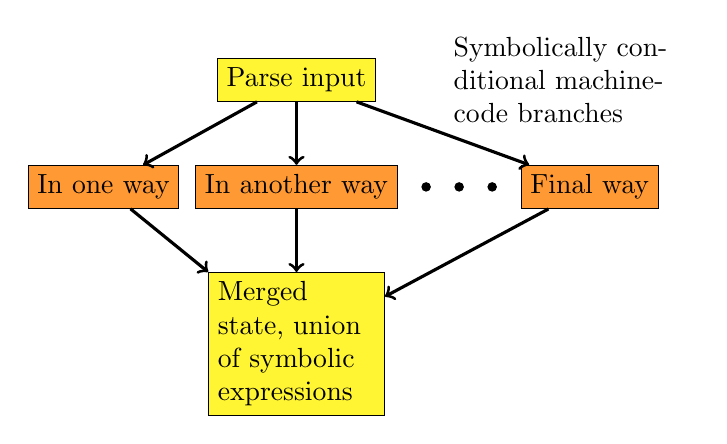
\begin{tikzpicture}

					\node [draw, fill=orange!80, minimum height=0.5cm]
					(first) {In one way};

					\node [draw, fill=orange!80, minimum height=0.5cm, right=0.2cm of first]
					(second) {In another way};

					\node [draw, fill=yellow!80, minimum
						width=1cm, minimum height=0.5cm, above=0.8cm of second]  (entry) {Parse input};

					\node [draw, circle, fill=black, minimum size=3pt, inner sep=0pt,
						right=0.3cm of second] (third) {};
					\node [draw, circle, fill=black, minimum size=3pt, inner sep=0pt,
						right=0.3cm of third] (fourth) {};
					\node [draw, circle, fill=black, minimum size=3pt, inner sep=0pt,
						right=0.3cm of fourth] (fifth) {};

					\node [draw, fill=orange!80, minimum height=0.5cm, right=0.3cm of fifth]
					(final) {Final way};

					\node [draw, fill=yellow!80, minimum height=0.5cm,
						below=0.8cm of second, text width=2cm ] (exit)
					{Merged state, union of symbolic expressions};

					\draw[->, line width=.4mm] (entry) to
					(first);
					\draw[->, line width=.4mm] (first) to (exit);

					\draw[->, line width=.4mm] (entry) to (second);
					\draw[->, line width=.4mm] (second) to (exit);

					\draw[->, line width=.4mm] (entry) to
					node[auto,text width=3cm]{Symbolically conditional machine-code branches}
					(final);
					\draw[->, line width=.4mm] (final) to (exit);

				\end{tikzpicture}
				\caption{State merging, schematic example}
			\end{figure}

		\end{column}
	\end{columns}
	\pause{}
	{\tiny
		\begin{figure}
			\begin{lstlisting}
(many lines elided)
..
getrandom("\xef\xd6\x9b\x35\x81\xc4\x7d\xb7", 8, GRND_NONBLOCK) = 8
brk(NULL)                               = 0x1700000
brk(0x1721000)                          = 0x1721000
read(0, "a\n", 4096)                    = 2
newfstatat(1, "", {st_mode=S_IFCHR|0620, st_rdev=makedev(0x88, 0x2), ...}, AT_EMPTY_PATH) = 0
write(1, "16\n", 3)                     = 3
lseek(0, -1, SEEK_CUR)                  = -1 ESPIPE (Illegal seek)
exit_group(0)                           = ?
+++ exited with 0 +++
\end{lstlisting}
			\caption{\texttt{echo 'a' | strace ./control-flow}}
		\end{figure}
	}
\end{frame}


\begin{frame}
	\begin{itemize}

		\item Fun idea for a tool, mostly novel

		\item Difficult to implement \& we were inexperienced

		\item The usefulness of the idea is validated

		\item AMBA is full of potential \& low-hanging fruit

	\end{itemize}
	\vfill
	\center{
		\url{https://github.com/lokegustafsson/amba/}
		\\
		(public after June 2nd 2023)
	}
\end{frame}


\end{document}
